\chapter{Clustering}

Wide ASPECS' well-defined, large cosmic volume allows for some of the first direct constraints on the clustering bias of CO emitters. This clustering bias can be then used to constrain the typical halo mass in which they reside \cite{10.1111/j.1365-2966.2011.20303.x}.

\section{Previous Work}

Previous work on clustering has been looked at different populations of galaxies. \cite{hickox2011clustering} looked at the clustering of quasars and obscured quasars. \cite{10.1111/j.1365-2966.2011.20303.x} looks at the clustering in SMGs and compares their clustering to clustering found for other sets of astronomical objects. 

\begin{figure}[tbp]
\centering 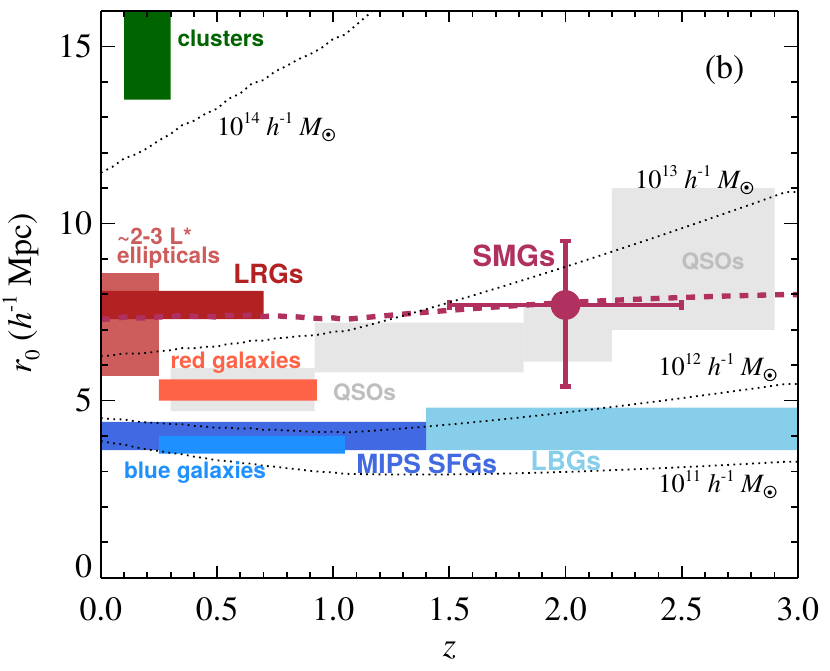
\includegraphics[width=120mm]{clustering/Hickox2012_Compare.png}
\caption{$r_0$ values for a variety of celestial objects as a function of redshift. Figure adapted from \cite{10.1111/j.1365-2966.2011.20303.x}.}
\label{fig:Hickox_compare}
\end{figure}

\section{Method}

\subsection{Angular Correlation Function}

The clustering is computed through a two point correlation function. The first step s to calculate the angular correlation function $ \omega(\theta)$. Once $ \omega(\theta)$ is computed, the second step is to obtain the two-point correlation function parameters of $r_0$ and $\gamma$.

The two-point correlation function, $\Eta(r)$, is the the probability of finding a galaxy at a separation $r$ from another randomly chosen galaxy in a volume $dV$ above Poisson, such that $$ dP = n[1 + \Eta(r)]dV$$, where $n$ is the mean space density of the galaxies in the sample\cite{hickox2011clustering}. 

To calculate the angular correlation function, the estimator from \cite{1993ApJ...412...64L} is used, where $$ \omega(\theta) = \frac{1}{RR}(DD-2DR + RR)$$, where $DD$, $DR$, and $RR$ are the number of data-data, data-random, and random-random galaxy pairs at a separation $\theta$, where each of the three collections is normalized to sum to 1 \cite{hickox2011clustering}.

Once the angular correlation function is found, a power-law model is fitted following $$\omega(\theta) = A\theta^{-\beta} $$ where $\beta$ = 0.8, a value used for many other galaxy angular correlations \cite{hickox2011clustering}.

\subsection{Obtaining $r_0$ and $\gamma$}

Two equations are used to convert the $A$ and $\beta$ to real-space $r_0$ and $\gamma$, 

$$ \gamma = \beta + 1 $$ and $$ A = H_{\gamma}\frac{\int_{0}^{\inf} (dN_1/dz)(dN_2/dz)E_z\chi^{1 - \gamma} dz}{[\int_{0}^{\inf} (dN_1/dz)dz][\int_{0}^{\inf} (dN_2/dz)dz]}r_0^{\gamma}$$

where $H_{\gamma} = \Gamma(0.5)\Gamma(0.5[\gamma -1])\Gamma(0.5\gamma)$, with $\Gamma$ being the gamma function, $\chi$ the radial comoving distance, $dN_{1,2}/dz$ are the redshift distributions of the samples, where in the case of autocorrelation are equal to each other, and $E_z = H_z/c = dz/d\chi$ \cite{hickox2011clustering}. The Hubble parameter $H_z$ can be found from
$$H_z^2 = H_0^2[\Omega_m(1+z)^3 + \Omega_{\lambda}]$$ \cite{hickox2011clustering}.

For this analysis, all CO line candidates above the 0.6 fidelity threshold were used, resulting in 35 sources, shown in Fig. \ref{fig:Clustering_points}. Two catalogs of random points were created, of 20000 points each, and their angular correlation computed to show that it is consistent with zero, shown in Fig.\ref{fig:random_points}. As a comparison, the two point correlation function was also computed for other fidelity cuts. The redshift distribution was taken from the CO redshifts of the lines, and the calculations were calculated over the range z = 1.5 to 3.5, as this is the range where most of the CO candidates seem to lie. To calculate $dN_{1,2}/dz$, the redshift distribution of the CO lines was fitted with a Gaussian, and the integral was taken over the Gaussian fit. The angular correlation function was computed over the range of 8.39 to 516.77 arcseconds, using logarithmically spaced bins. 

% Random points: 582.10 arcseconds, DD points, 516 arcseconds

\begin{figure}[tbp]
\centering 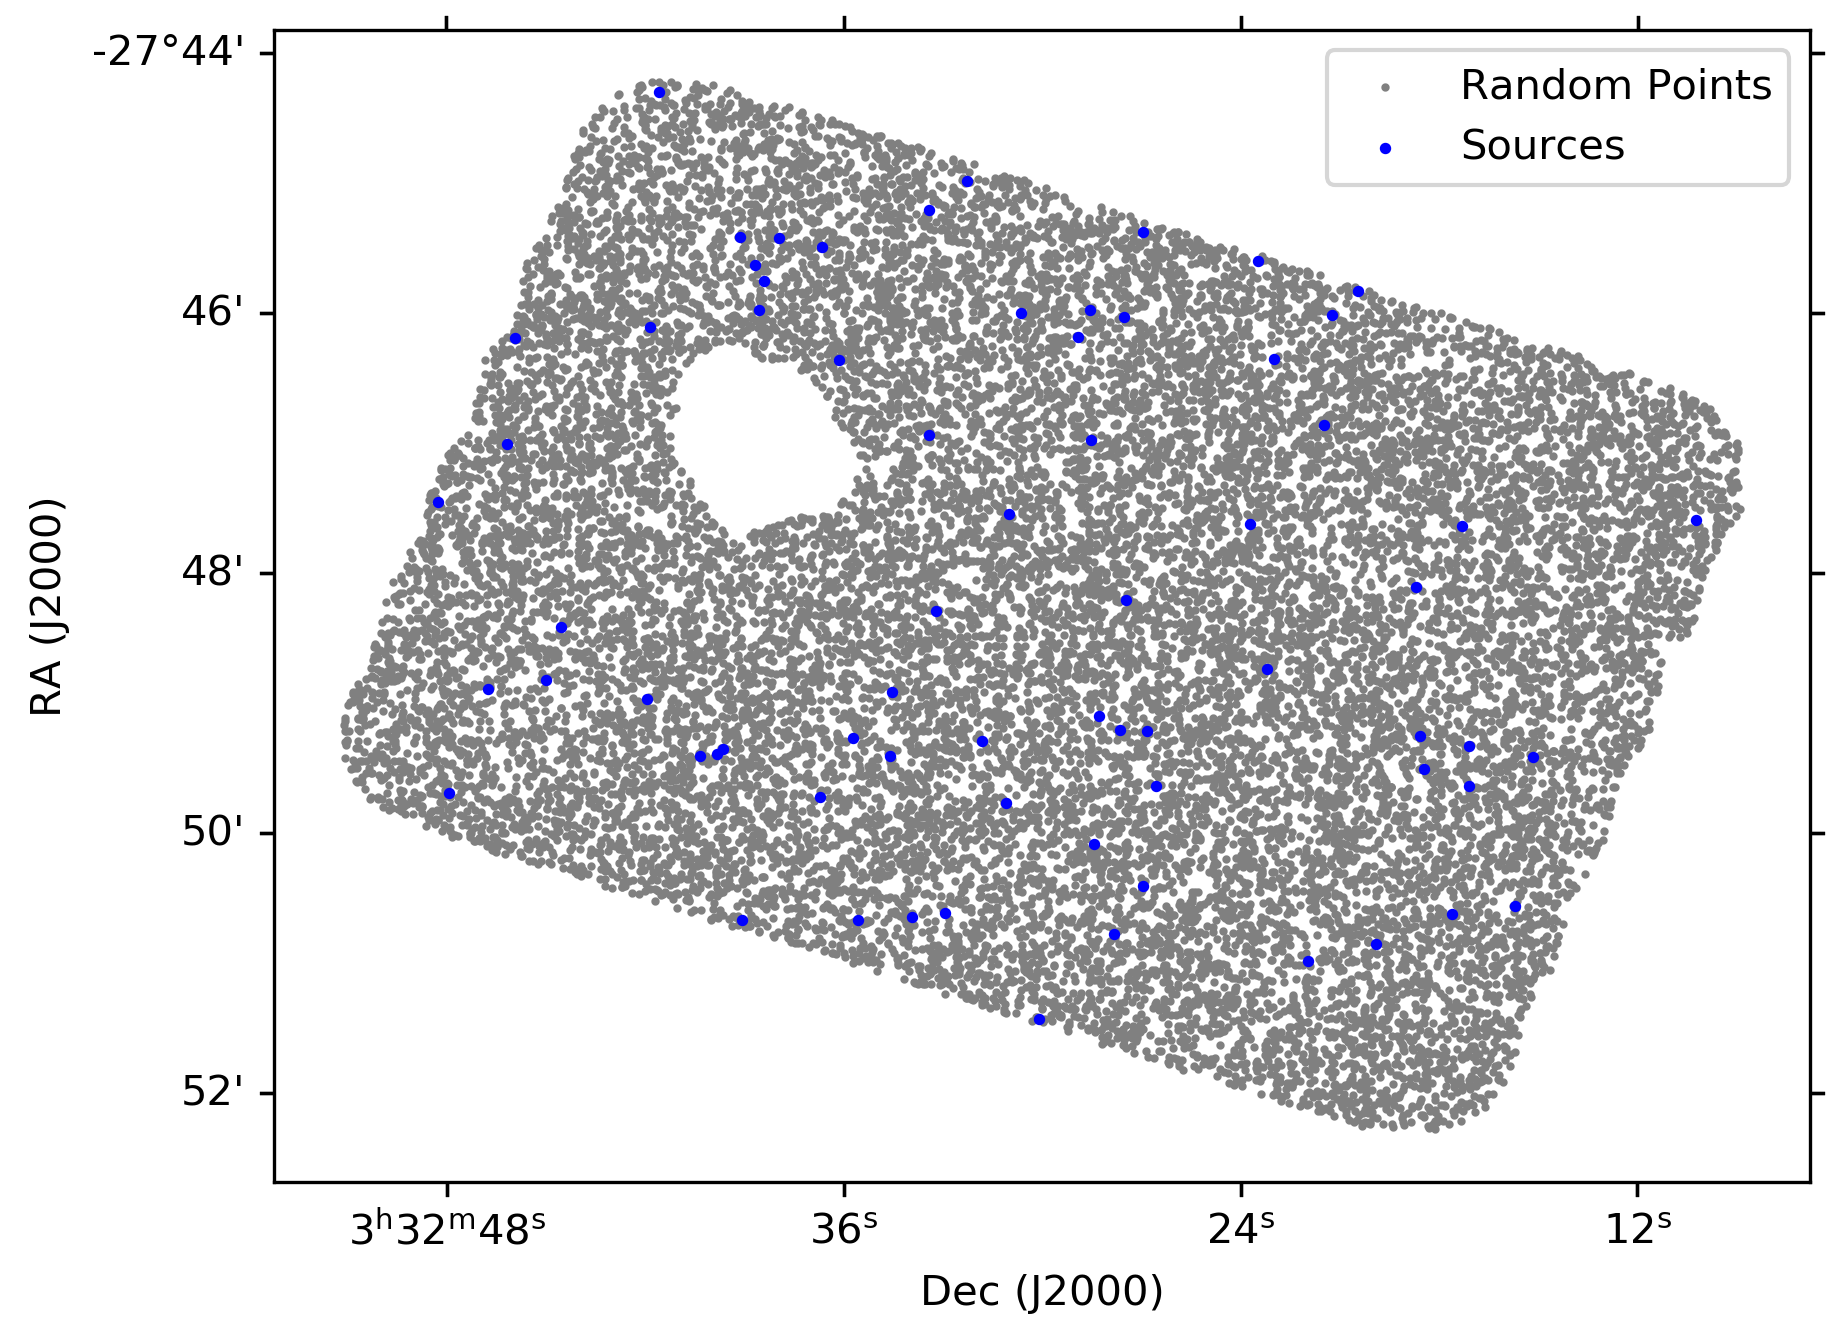
\includegraphics[width=120mm]{PDFS/NX_V_Y_Sources_20000.png}
\caption{Random points and sources from the $>$ 0.6 fidelity cut. The random points are distributed uniformly throughout the Wide ASPECS footprint.}
\label{fig:Clustering_points}
\end{figure}

\begin{figure}[tbp]
\centering 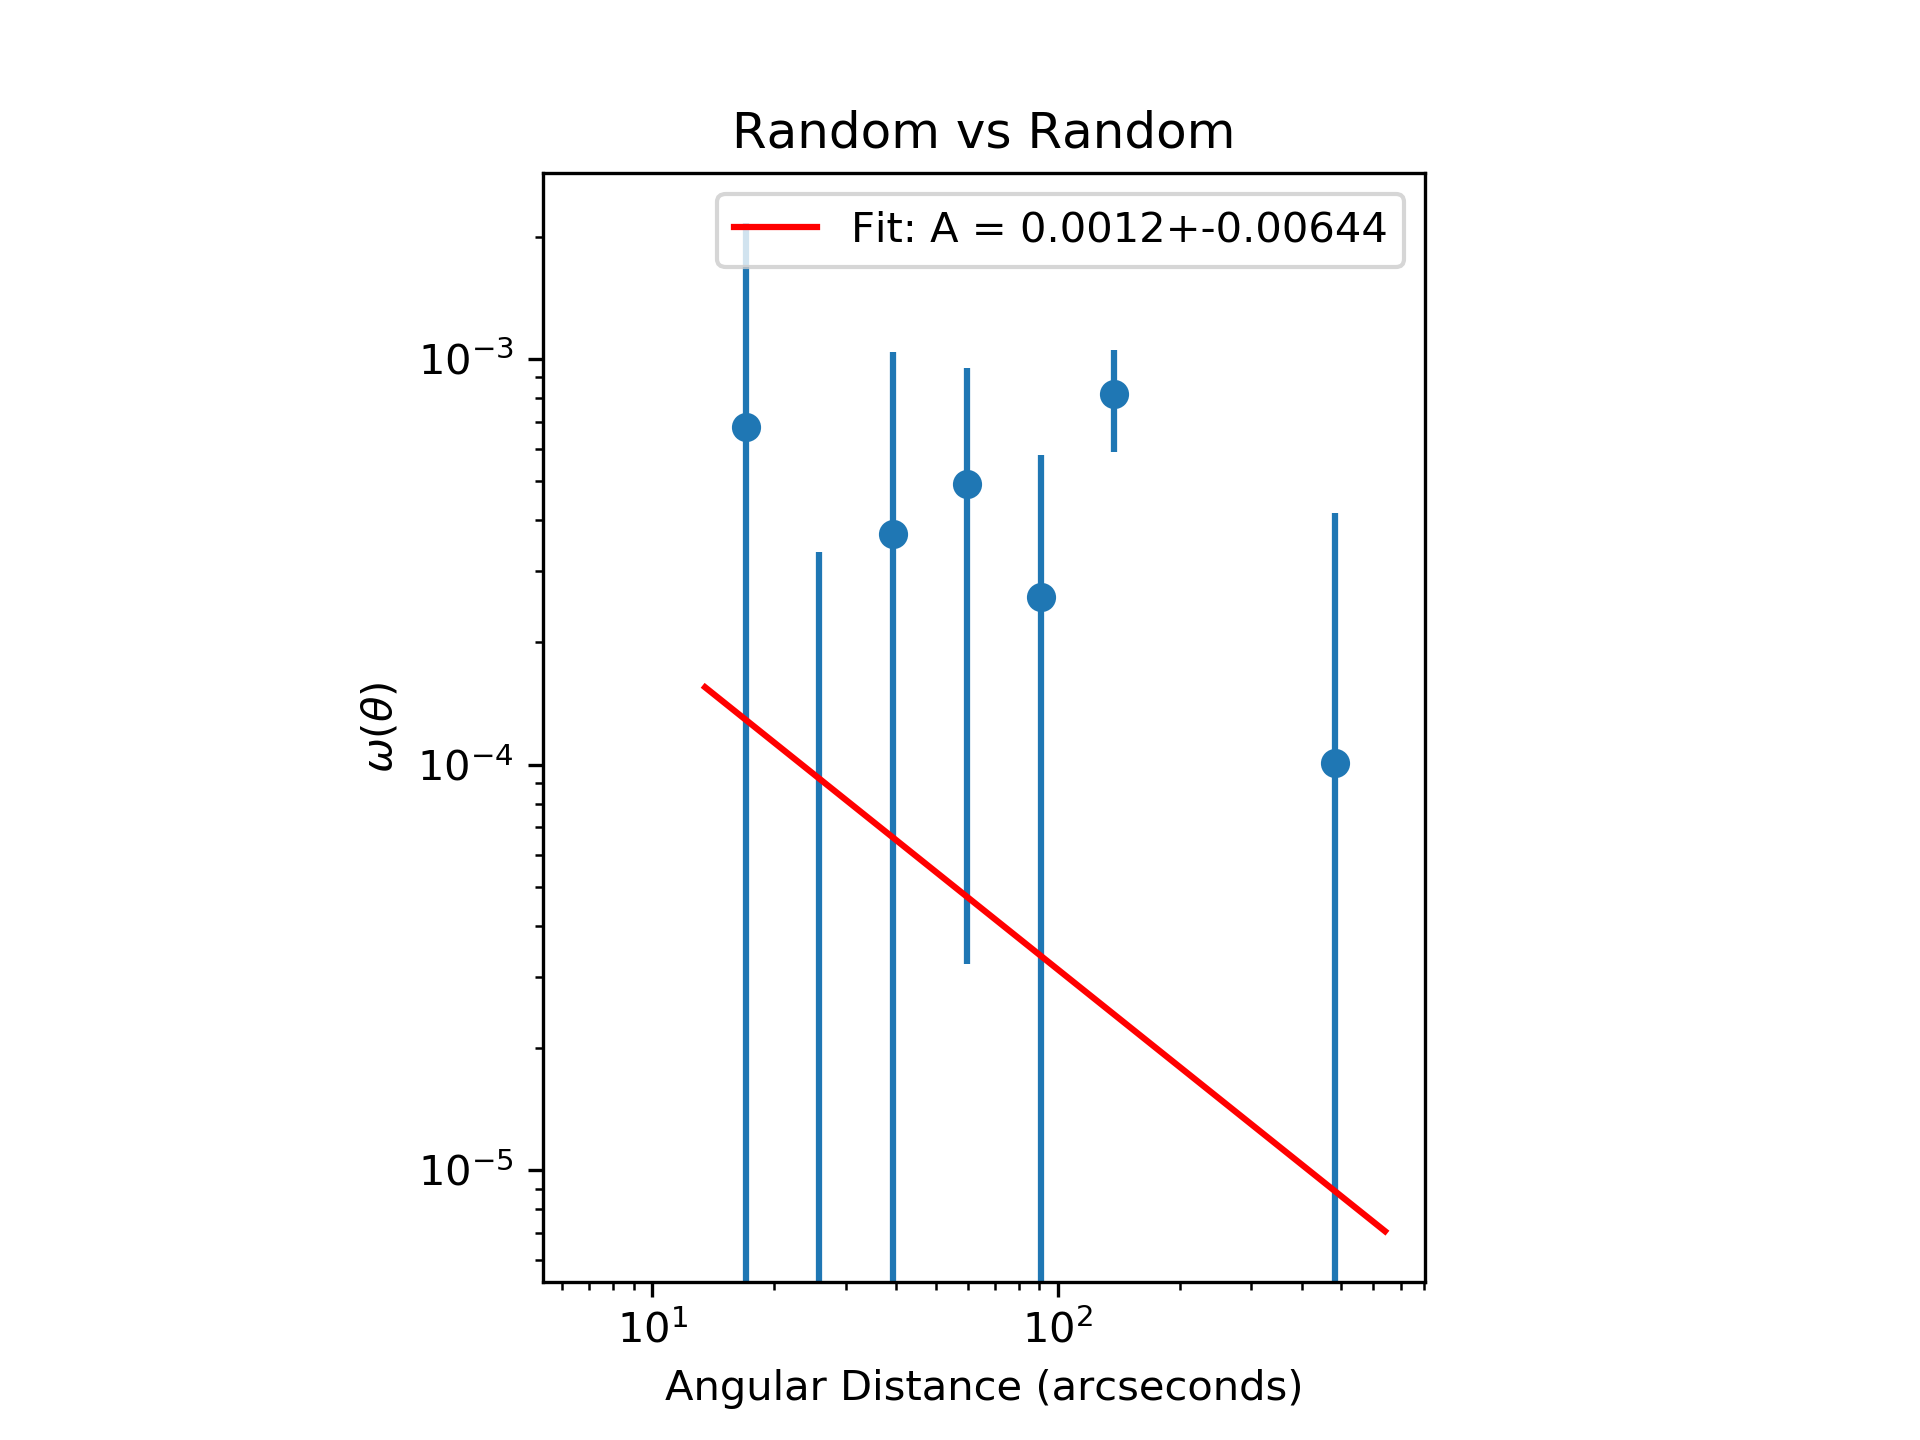
\includegraphics[width=60mm]{clustering/Log_Random_vs_Random_15000NoParenFlip_bin10.png}
\caption{Angular correlation two sets of random points used in this analysis, showing that the angular correlation is consistent with zero, as would be expected for uniformly distributed points.}
\label{fig:random_points}
\end{figure}

\section{Results}

As can be seen in Fig. \ref{fig:Angular_correlation}, as the fidelity increases, $A$ increases as well. The change is most significant when only fitting the positive points.  When converted to $r_0$, the fidelity cuts result in $r_0$ values of 23 +- 5 for fidelity $>$ 0.7, 20 +- 2 for fidelity $>$ 0.6, 8 +- 1.5 for fidelity $>$ 0.5, and no $r_0$ for fidelity > 0.4, as the $A$ value is consistent with 0. 

\begin{figure}[tbp]
\centering 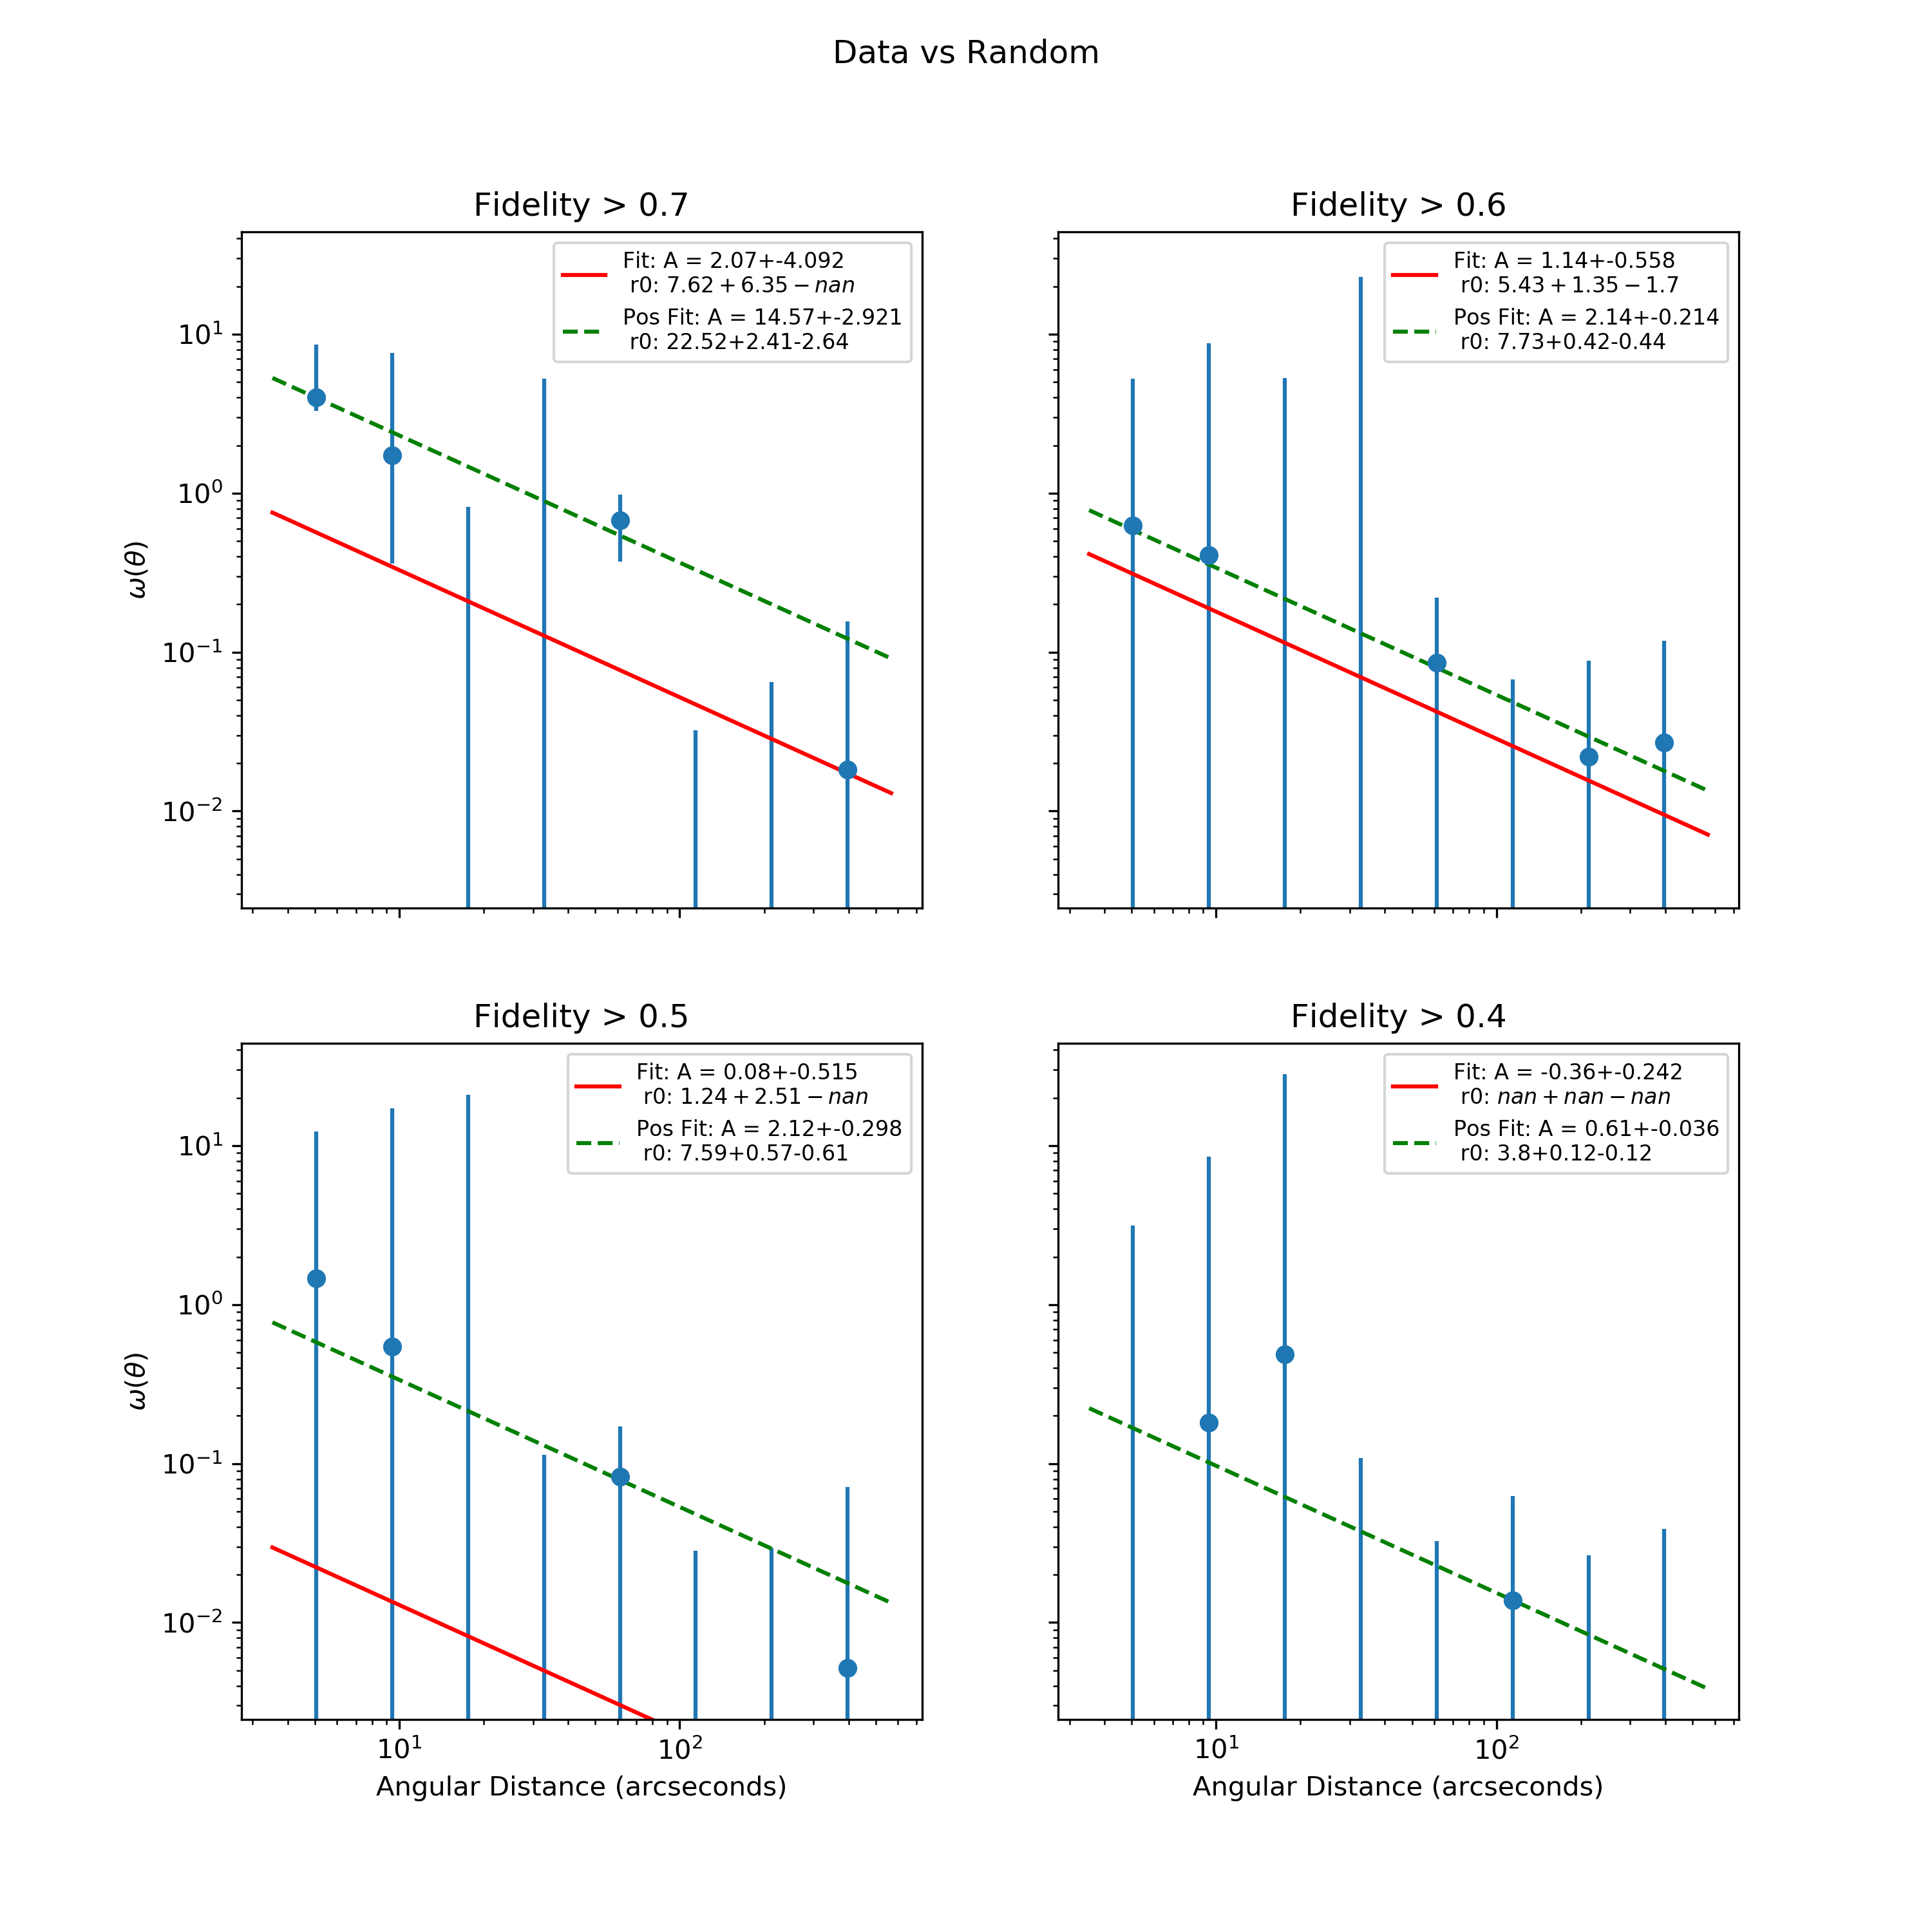
\includegraphics[width=120mm]{Log_4Panel_Data_Vs_Random_bin8_NFalse_Num10000.png}
\caption{Angular correlation function for various fidelity cuts. The bins increase logarithmically from 8.39 arcsecs to 516.77 arcseconds. The red lines are from fitting $\omega(\theta) = A\theta^{-0.8} $ to all of the bins. The green dashed line is from fitting that same equation only to bins that had a positive value. As the fidelity goes up, the $A$ value increases as well, indicating stronger clustering. The few line candidates means that the results are quite noisy, and are sensitive to the bins chosen.}
\label{fig:Angular_correlation}
\end{figure}

Besides the different fidelity cuts, different binnings also are included to study their effects on the final $r_0$ results. The results seem to be very dependent on the binning. While the values for the only positively fitted bins does not change dramatically as the binning changes, the number of bins does make a large difference in the final $A$, and therefore $r_0$ values, as can be seen in Figures \ref{fig:Angular_bin_10} and \ref{fig:Angular_bin_8}.

\begin{figure}[!tbp]
\centering 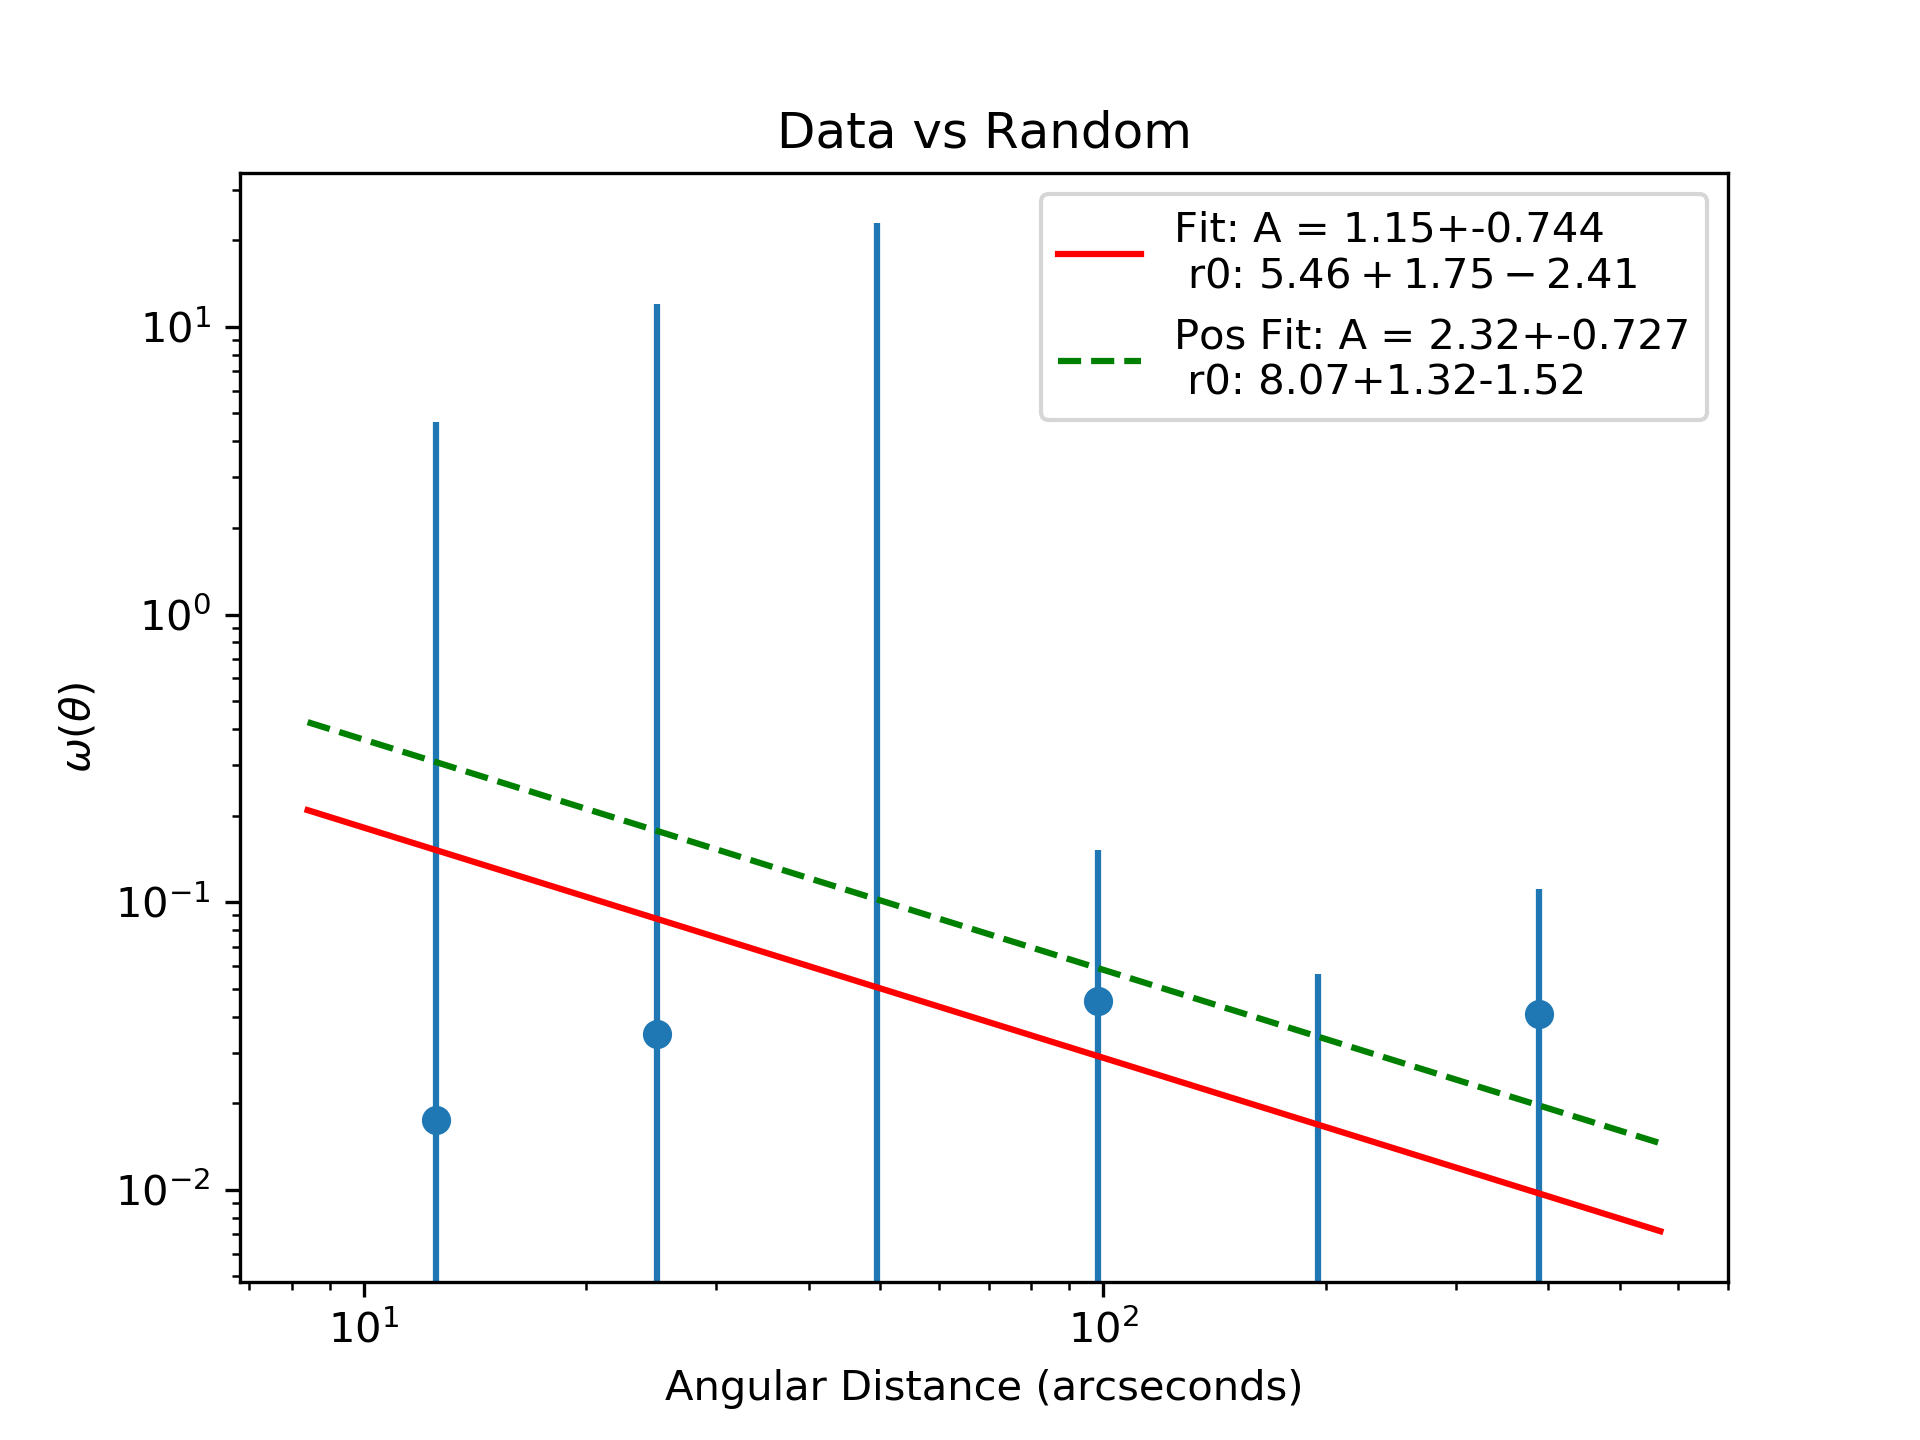
\includegraphics[width=90mm]{Data_vs_Random_10000_bin6_sn0_6_NFalse.png}
\caption{Angular correlation function for 6 bins for the chosen fidelity cut of 0.6. Red is the fit $\omega(\theta) = A\theta^{-0.8}$ to all the bins, while the green line is the fit to only the positive bins. This is the final binning used for the analysis. }
\label{fig:Angular_binnings}
\end{figure}

\begin{figure}[!tbp]
\centering 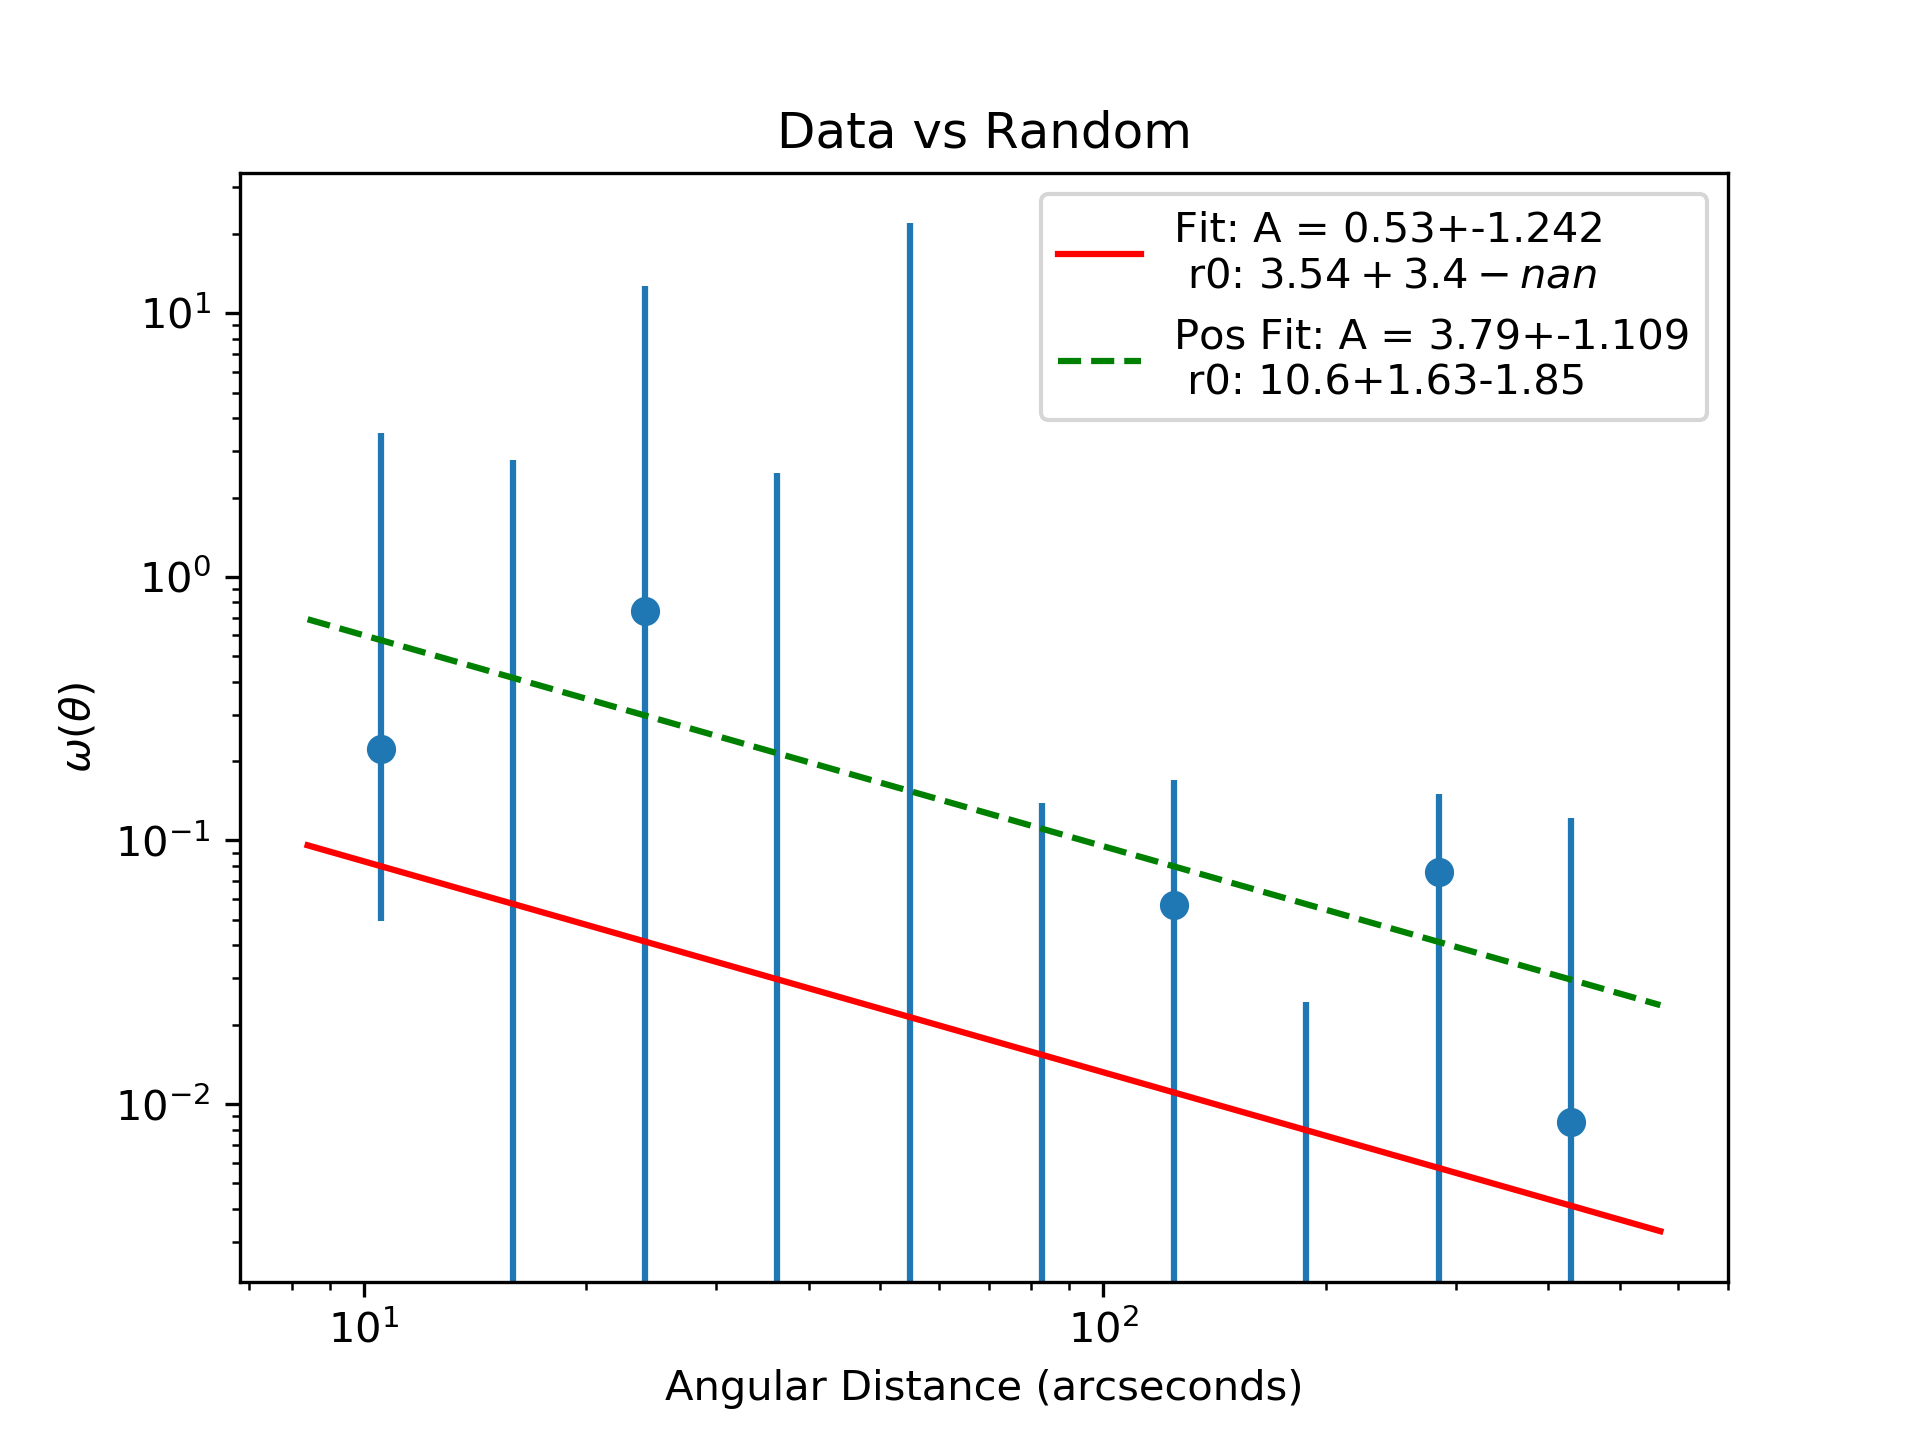
\includegraphics[width=90mm]{Data_vs_Random_10000_bin10_sn0_6_NFalse.png}
\caption{Angular correlation function for 10 bins  for fidelity $>$ 0.6.}
\label{fig:Angular_bin_10}
\end{figure}

\begin{figure}[!tbp]
\centering 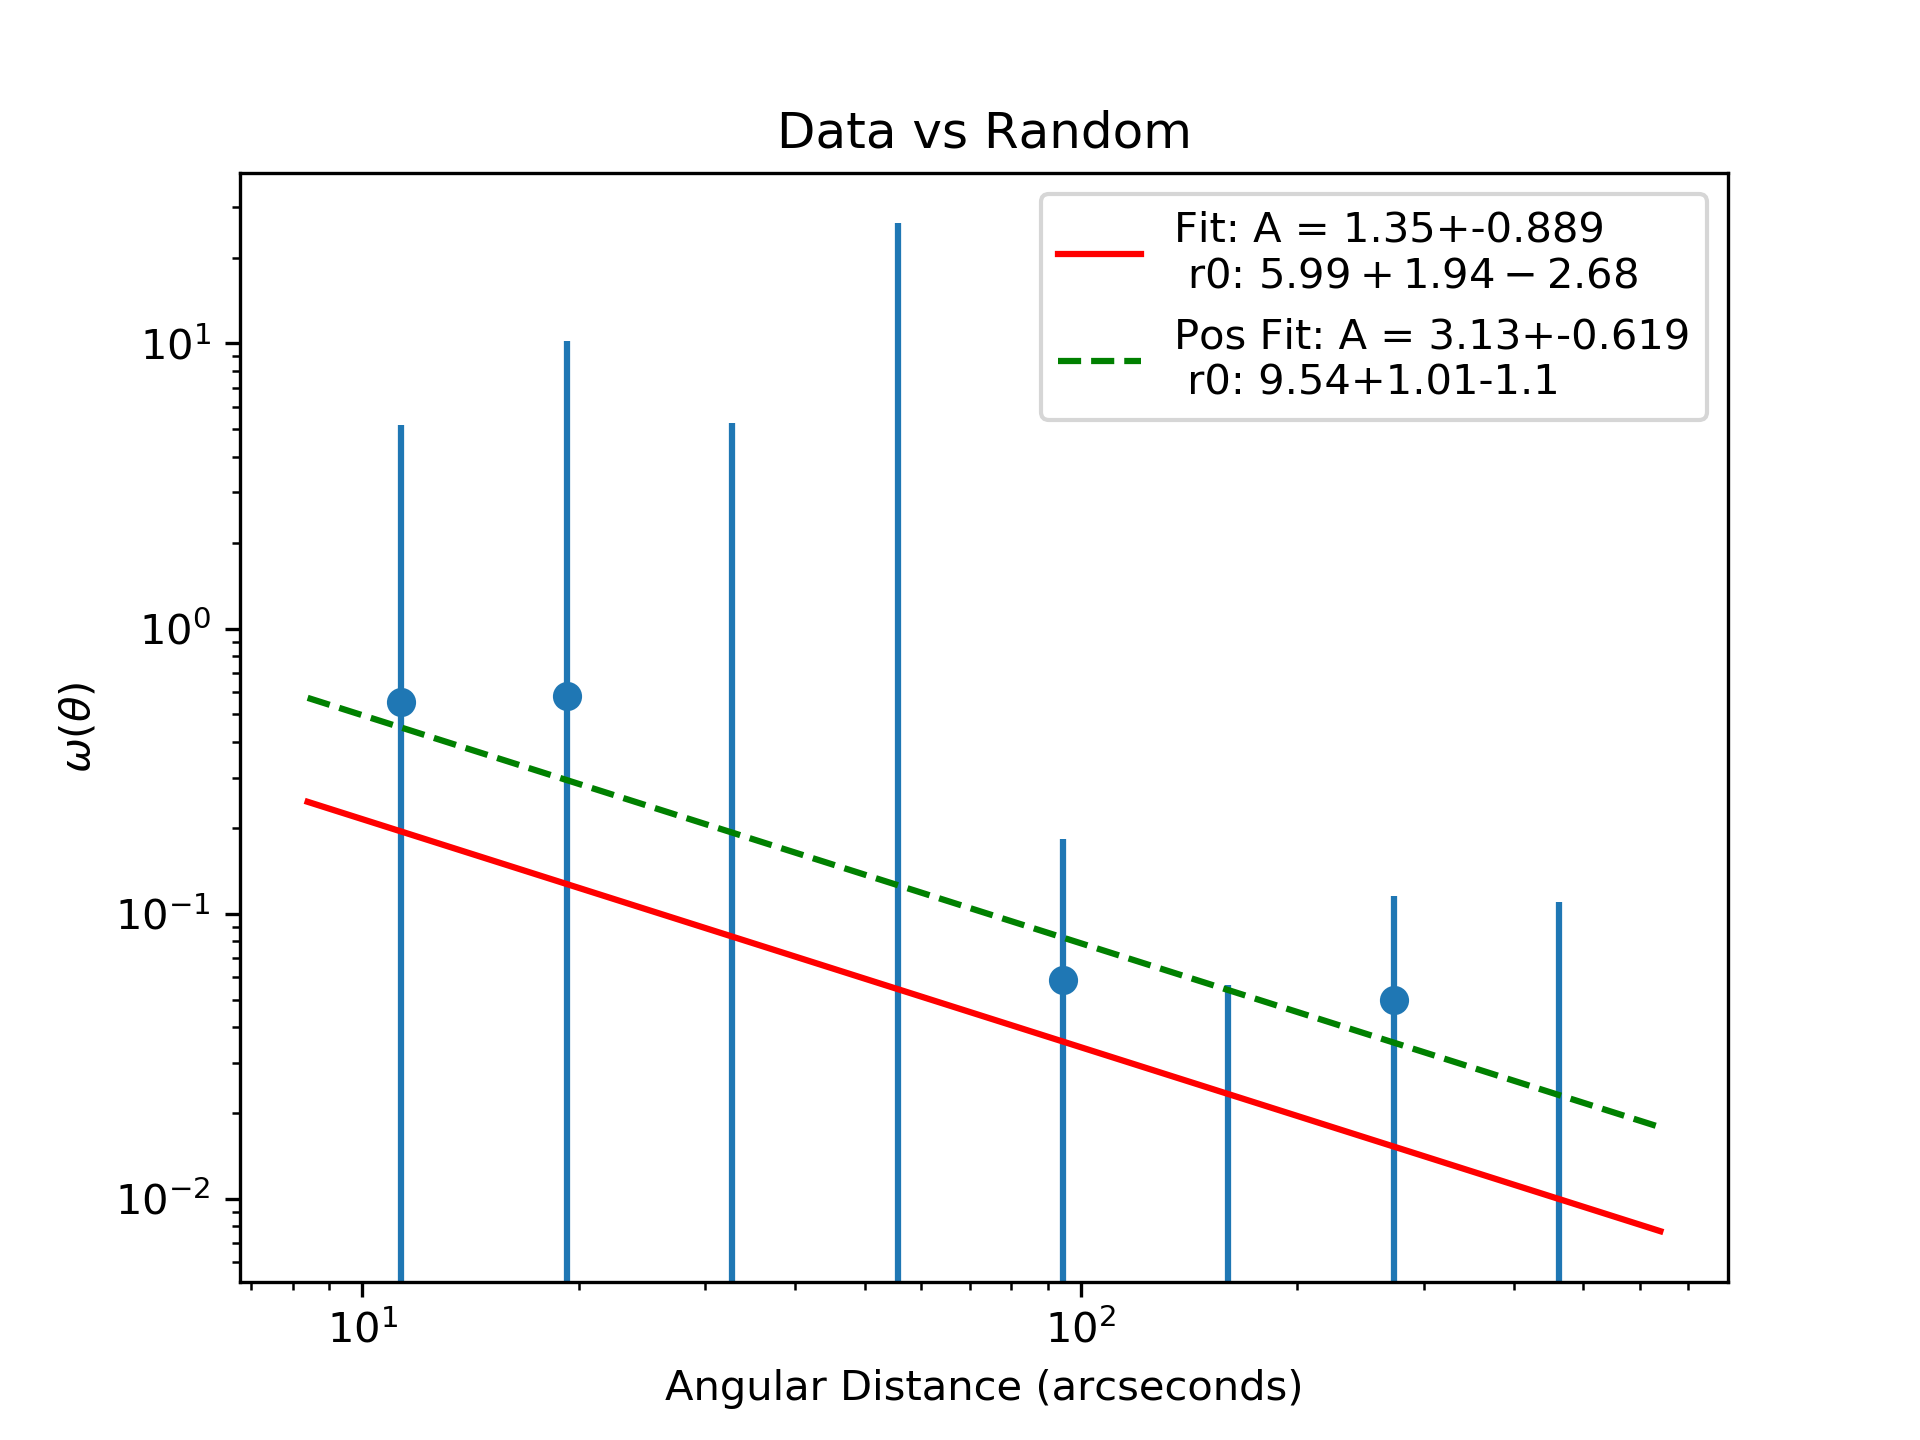
\includegraphics[width=90mm]{Data_vs_Random_10000_bin8_sn0_6_NFalse.png}
\caption{Angular correlation function for 8 bins for fidelity $>$ 0.6.}
\label{fig:Angular_bin_8}
\end{figure}

As should be expected, as the fidelity cut goes up, meaning a larger portion of the CO lines remaining are true sources, the clustering value becomes larger as well. Once the fidelity drops below 0.5, such that the majority of the lines should be false positives, the clustering values drop to be consistent with 0.

\section{Discussion}

The clustering results do show that there is a larger $r_0$ as the fidelity cut becomes higher, suggesting that there are real sources in the sample. On the other hand, the clustering measurement is still very noisy and future work will be required to get a better final clustering measurement. 

In comparison to other clustering measurements, \cite{hickox2011clustering} found an $r_0$ for quasers to be between 5.5 and 

\cite{hickox2011clustering} showed that for SMG galaxies, around a redshift of 2, the autocorrelation length $r_0 \approx 6 h^{-1} Mpc$. For the 35 sources used here, a slightly higher, but similar $r_0$ has been found. 

